\documentclass[aspectratio=169]{beamer}

\usetheme{Madrid}
\usecolortheme{default}

\usepackage{tikz}
\usepackage{booktabs}
\usepackage{amsmath}
\usetikzlibrary{arrows.meta, positioning, shapes.geometric}

\title{The Byzantine Generals Problem}
\subtitle{Understanding Byzantine Faults and OM($m$)}
\author{Your Name}
\date{\today}

\begin{document}

%------------------------------------------------
\begin{frame}
  \titlepage
\end{frame}

%------------------------------------------------
\begin{frame}{Presentation Overview}
\begin{itemize}
  \item Motivation: why Byzantine faults matter
  \item The Byzantine Generals Problem
  \item Interactive consistency
  \item Why three generals are not enough
  \item OM($m$): Oral Messages algorithm
  \item Connection to PBFT
\end{itemize}
\end{frame}

%------------------------------------------------
\begin{frame}{Crash Fault vs Byzantine Fault}

\begin{columns}

\column{0.48\textwidth}
\begin{block}{Crash Fault}
\centering
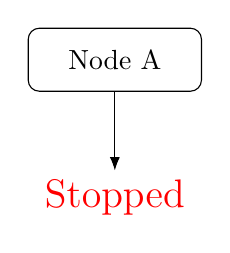
\begin{tikzpicture}[node distance=1cm]
\node[draw, rounded corners, minimum width=2.2cm, minimum height=0.8cm] (a) {Node A};
\node[below=of a, text=red] (stop) {\Large Stopped};
\draw[-{Latex}] (a) -- (stop);
\end{tikzpicture}

\vspace{0.3cm}
\begin{itemize}
  \item Node stops responding
  \item Easier to detect
  \item Paxos / Raft mainly assume this model
\end{itemize}
\end{block}

\column{0.48\textwidth}
\begin{alertblock}{Byzantine Fault}
\centering
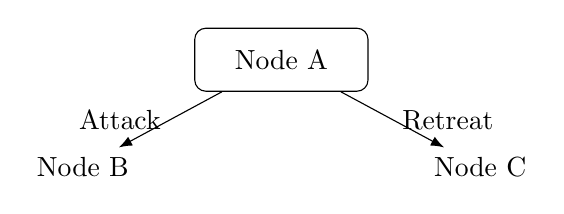
\begin{tikzpicture}[node distance=1cm]
\node[draw, rounded corners, minimum width=2.2cm, minimum height=0.8cm] (a) {Node A};
\node[below left=of a] (b) {Node B};
\node[below right=of a] (c) {Node C};
\draw[-{Latex}] (a) -- node[left] {Attack} (b);
\draw[-{Latex}] (a) -- node[right] {Retreat} (c);
\end{tikzpicture}

\vspace{0.3cm}
\begin{itemize}
  \item Node may lie
  \item Sends inconsistent messages
  \item Much harder to tolerate
\end{itemize}
\end{alertblock}

\end{columns}

\end{frame}

%------------------------------------------------
\begin{frame}{The Byzantine Generals Problem}

\begin{center}
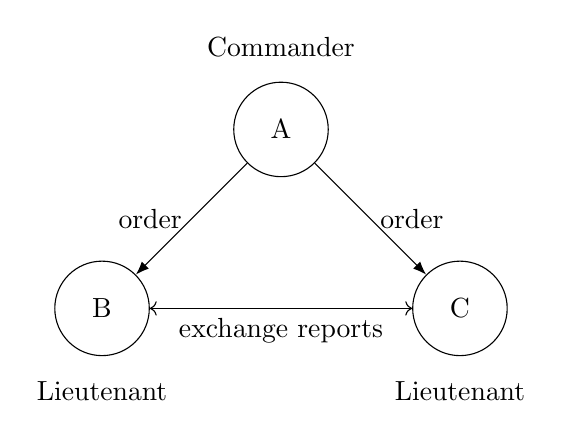
\begin{tikzpicture}[node distance=2cm]
\node[draw, circle, minimum size=1.2cm] (A) {A};
\node[draw, circle, below left=of A, minimum size=1.2cm] (B) {B};
\node[draw, circle, below right=of A, minimum size=1.2cm] (C) {C};

\draw[-{Latex}] (A) -- node[left] {order} (B);
\draw[-{Latex}] (A) -- node[right] {order} (C);
\draw[<->] (B) -- node[below] {exchange reports} (C);

\node[above=0.2cm of A] {Commander};
\node[below=0.2cm of B] {Lieutenant};
\node[below=0.2cm of C] {Lieutenant};
\end{tikzpicture}
\end{center}

\begin{block}{Goal}
All loyal generals must choose the same action: \textbf{Attack} or \textbf{Retreat}.
\end{block}

\end{frame}

%------------------------------------------------
\begin{frame}{Interactive Consistency}

\begin{columns}

\column{0.48\textwidth}
\begin{block}{IC1: Agreement}
All loyal lieutenants obey the same order.

\vspace{0.4cm}
\centering
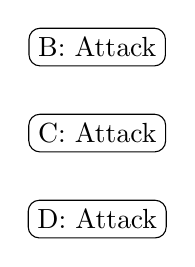
\begin{tikzpicture}
\node[draw, rounded corners] (b) {B: Attack};
\node[draw, rounded corners, below=0.6cm of b] (c) {C: Attack};
\node[draw, rounded corners, below=0.6cm of c] (d) {D: Attack};
\end{tikzpicture}
\end{block}

\column{0.48\textwidth}
\begin{block}{IC2: Validity}
If the commander is loyal, every loyal lieutenant follows the commander's order.

\vspace{0.4cm}
\centering
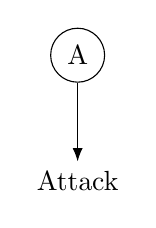
\begin{tikzpicture}[node distance=1cm]
\node[draw, circle] (a) {A};
\node[below=of a] (cmd) {Attack};
\draw[-{Latex}] (a) -- (cmd);
\end{tikzpicture}
\end{block}

\end{columns}

\end{frame}

%------------------------------------------------
\begin{frame}{Why Three Generals Are Impossible}

\begin{center}
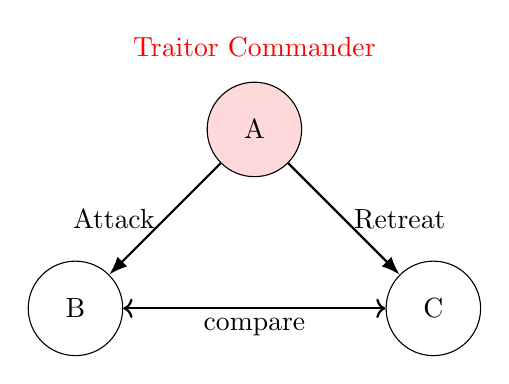
\begin{tikzpicture}[node distance=2cm]
\node[draw, circle, fill=red!15, minimum size=1.2cm] (A) {A};
\node[draw, circle, below left=of A, minimum size=1.2cm] (B) {B};
\node[draw, circle, below right=of A, minimum size=1.2cm] (C) {C};

\draw[-{Latex}, thick] (A) -- node[left] {Attack} (B);
\draw[-{Latex}, thick] (A) -- node[right] {Retreat} (C);
\draw[<->, thick] (B) -- node[below] {compare} (C);

\node[above=0.2cm of A, text=red] {Traitor Commander};
\end{tikzpicture}
\end{center}

\begin{alertblock}{Problem}
B sees ``Attack'' from A and ``Retreat'' from C.  
B cannot distinguish whether A is lying or C is lying.
\end{alertblock}

\end{frame}

%------------------------------------------------
\begin{frame}{Information Ambiguity}

\begin{table}
\centering
\begin{tabular}{lll}
\toprule
World & B's Observation & Possible Explanation \\
\midrule
World 1 & A says Attack, C says Retreat & A is traitor \\
World 2 & A says Attack, C says Retreat & C is traitor \\
\bottomrule
\end{tabular}
\end{table}

\vspace{0.4cm}

\begin{block}{Key Insight}
The loyal general cannot distinguish two different worlds from the same local information.
\end{block}

\begin{alertblock}{Conclusion}
With three generals and one traitor, no algorithm can guarantee both IC1 and IC2.
\end{alertblock}

\end{frame}

%------------------------------------------------
\begin{frame}{How Many Generals Are Needed?}

\begin{columns}

\column{0.48\textwidth}
\begin{block}{Required Number}
To tolerate $m$ Byzantine traitors:

\[
n \ge 3m + 1
\]

\end{block}

\column{0.48\textwidth}
\begin{table}
\centering
\begin{tabular}{cc}
\toprule
Traitors $m$ & Required Generals \\
\midrule
0 & 1 \\
1 & 4 \\
2 & 7 \\
3 & 10 \\
\bottomrule
\end{tabular}
\end{table}

\end{columns}

\vspace{0.4cm}

\begin{alertblock}{Connection}
PBFT uses the same principle: to tolerate $f$ Byzantine replicas, it requires $3f+1$ replicas.
\end{alertblock}

\end{frame}

%------------------------------------------------
\begin{frame}{OM(0): No Traitors}

\begin{center}
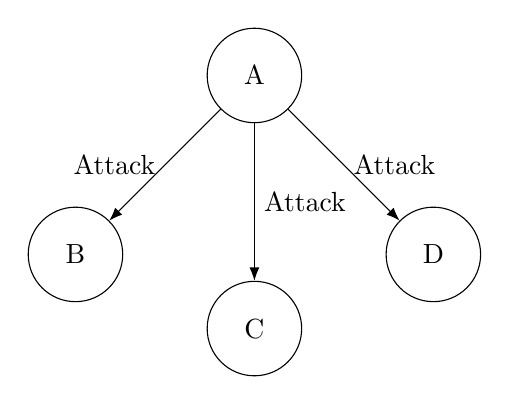
\begin{tikzpicture}[node distance=2cm]
\node[draw, circle, minimum size=1.2cm] (A) {A};
\node[draw, circle, below left=of A, minimum size=1.2cm] (B) {B};
\node[draw, circle, below=of A, minimum size=1.2cm] (C) {C};
\node[draw, circle, below right=of A, minimum size=1.2cm] (D) {D};

\draw[-{Latex}] (A) -- node[left] {Attack} (B);
\draw[-{Latex}] (A) -- node[right] {Attack} (C);
\draw[-{Latex}] (A) -- node[right] {Attack} (D);
\end{tikzpicture}
\end{center}

\begin{block}{OM(0)}
The commander sends a value, and each lieutenant adopts the received value.
\end{block}

\end{frame}

%------------------------------------------------
\begin{frame}{OM(1): One Traitor}

\begin{center}
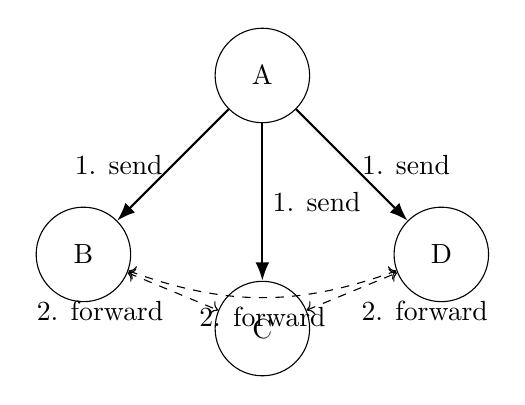
\begin{tikzpicture}[node distance=2cm]
\node[draw, circle, minimum size=1.2cm] (A) {A};
\node[draw, circle, below left=of A, minimum size=1.2cm] (B) {B};
\node[draw, circle, below=of A, minimum size=1.2cm] (C) {C};
\node[draw, circle, below right=of A, minimum size=1.2cm] (D) {D};

\draw[-{Latex}, thick] (A) -- node[left] {1. send} (B);
\draw[-{Latex}, thick] (A) -- node[right] {1. send} (C);
\draw[-{Latex}, thick] (A) -- node[right] {1. send} (D);

\draw[<->, dashed] (B) -- node[below left] {2. forward} (C);
\draw[<->, dashed] (C) -- node[below right] {2. forward} (D);
\draw[<->, dashed] (B) to[bend right=20] node[below] {2. forward} (D);
\end{tikzpicture}
\end{center}

\begin{block}{OM(1)}
Each lieutenant forwards what it received, then takes a majority vote.
\end{block}

\end{frame}

%------------------------------------------------
\begin{frame}{OM(1) Example: Commander Is Traitor}

\begin{center}
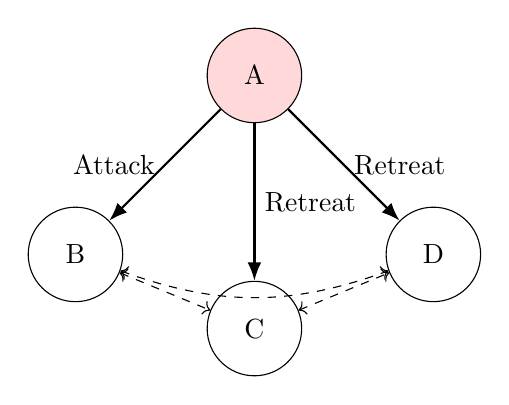
\begin{tikzpicture}[node distance=2cm]
\node[draw, circle, fill=red!15, minimum size=1.2cm] (A) {A};
\node[draw, circle, below left=of A, minimum size=1.2cm] (B) {B};
\node[draw, circle, below=of A, minimum size=1.2cm] (C) {C};
\node[draw, circle, below right=of A, minimum size=1.2cm] (D) {D};

\draw[-{Latex}, thick] (A) -- node[left] {Attack} (B);
\draw[-{Latex}, thick] (A) -- node[right] {Retreat} (C);
\draw[-{Latex}, thick] (A) -- node[right] {Retreat} (D);

\draw[<->, dashed] (B) -- (C);
\draw[<->, dashed] (C) -- (D);
\draw[<->, dashed] (B) to[bend right=20] (D);
\end{tikzpicture}
\end{center}

\begin{table}
\centering
\begin{tabular}{c c c c c}
\toprule
Lieutenant & Direct & From B & From C & Decision \\
\midrule
B & Attack & -- & Retreat & Retreat \\
C & Retreat & Attack & -- & Retreat \\
D & Retreat & Attack & Retreat & Retreat \\
\bottomrule
\end{tabular}
\end{table}

\end{frame}

%------------------------------------------------
\begin{frame}{General Form of OM($m$)}

\begin{center}
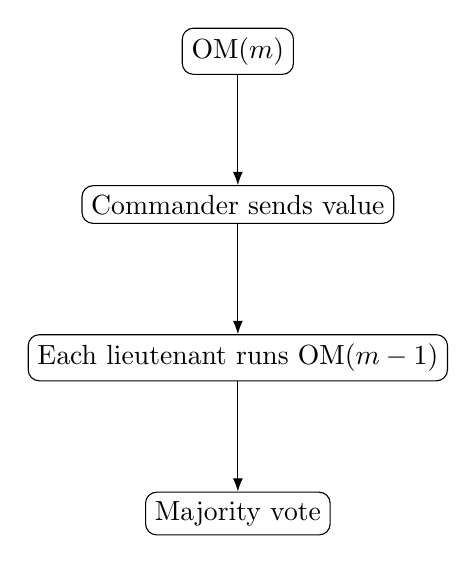
\begin{tikzpicture}[node distance=1.4cm]
\node[draw, rounded corners] (om2) {OM($m$)};
\node[draw, rounded corners, below=of om2] (send) {Commander sends value};
\node[draw, rounded corners, below=of send] (rec) {Each lieutenant runs OM($m-1$)};
\node[draw, rounded corners, below=of rec] (maj) {Majority vote};

\draw[-{Latex}] (om2) -- (send);
\draw[-{Latex}] (send) -- (rec);
\draw[-{Latex}] (rec) -- (maj);
\end{tikzpicture}
\end{center}

\begin{block}{Recursive Structure}
OM($m$) solves the problem by reducing it to smaller OM($m-1$) problems.
\end{block}

\end{frame}

%------------------------------------------------
\begin{frame}{Message Depth in OM($m$)}

\begin{table}
\centering
\begin{tabular}{ccc}
\toprule
Algorithm & Faults Tolerated & Message Depth \\
\midrule
OM(0) & 0 & 1 step \\
OM(1) & 1 & 2 steps \\
OM(2) & 2 & 3 steps \\
OM($m$) & $m$ & $m+1$ steps \\
\bottomrule
\end{tabular}
\end{table}

\vspace{0.4cm}

\begin{block}{Intuition}
More Byzantine faults require deeper message forwarding, because loyal nodes need more evidence from multiple paths.
\end{block}

\end{frame}

%------------------------------------------------
\begin{frame}{From Byzantine Generals to PBFT}

\begin{center}
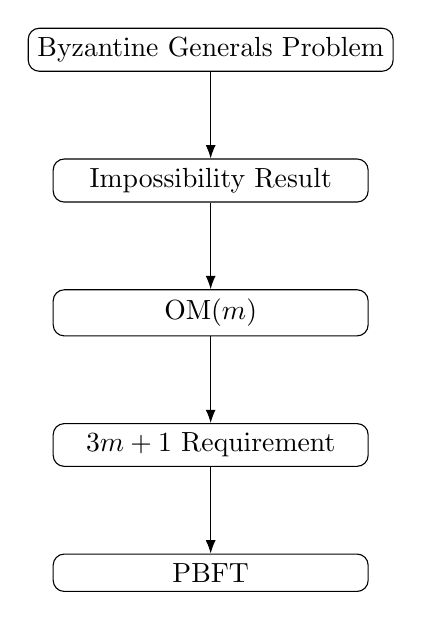
\begin{tikzpicture}[node distance=1.1cm]
\node[draw, rounded corners, minimum width=4cm] (bgp) {Byzantine Generals Problem};
\node[draw, rounded corners, below=of bgp, minimum width=4cm] (imposs) {Impossibility Result};
\node[draw, rounded corners, below=of imposs, minimum width=4cm] (om) {OM($m$)};
\node[draw, rounded corners, below=of om, minimum width=4cm] (rule) {$3m+1$ Requirement};
\node[draw, rounded corners, below=of rule, minimum width=4cm] (pbft) {PBFT};

\draw[-{Latex}] (bgp) -- (imposs);
\draw[-{Latex}] (imposs) -- (om);
\draw[-{Latex}] (om) -- (rule);
\draw[-{Latex}] (rule) -- (pbft);
\end{tikzpicture}
\end{center}

\end{frame}

%------------------------------------------------
\begin{frame}{PBFT Interprets the Theory Practically}

\begin{columns}

\column{0.48\textwidth}
\begin{block}{Byzantine Generals}
\begin{itemize}
  \item Theoretical model
  \item Oral messages
  \item Recursive forwarding
  \item Agreement among loyal generals
\end{itemize}
\end{block}

\column{0.48\textwidth}
\begin{block}{PBFT}
\begin{itemize}
  \item Practical replicated service
  \item Pre-prepare
  \item Prepare
  \item Commit
  \item View change
\end{itemize}
\end{block}

\end{columns}

\vspace{0.4cm}

\begin{alertblock}{Key Difference}
PBFT is not just majority voting. It orders client requests safely in a real distributed system.
\end{alertblock}

\end{frame}

%------------------------------------------------
\begin{frame}{Takeaways}

\begin{itemize}
  \item Byzantine faults are stronger than crash faults.
  \item The goal is agreement among loyal nodes, not necessarily identifying traitors.
  \item With three generals and one traitor, agreement is impossible.
  \item OM($m$) uses recursive message forwarding and majority voting.
  \item To tolerate $m$ Byzantine faults, at least $3m+1$ generals are required.
  \item PBFT builds on this theory to implement practical Byzantine fault-tolerant replication.
\end{itemize}

\end{frame}

\end{document}